\chapter{Experiments and Results}
\label{chap:exp}
 
\section{Datasets}

The parallel implementation of Subgraph Isomorphism Algorithm has been compared to sequential implementation of VF2 algorithm on various real world datasets. Following is a brief overview of the datasets that have been used to perform experiments.

\begin{table}[h!]
  \begin{center}
    \caption{Datasets}
    \label{tab:table1}
    \begin{tabular}{l||l|l} % <-- Alignments: 1st column left, 2nd middle and 3rd right, with vertical lines in between
      \textbf{Dataset} & \textbf{Vertices} & \textbf{Edges}\\
      \hline
      Jazz musicians & 198 & 2742\\
      Facebook (NIPS) & 2888 & 2981\\
      	U. Rovira i Virgili & 1133 & 5451\\
      	Hamsterster friendships & 1858 & 12534\\
      	US power grid & 4941 & 6594\\
      	Chicago transporation & 1467 & 1298
    \end{tabular}
  \end{center}
\end{table}

For these datasets, random connected query graphs are generated to run the algorithm. To generate labelled graphs, labels are randomly allotted to the vertices of the data and query graphs.

\section{Dataset: Jazz Musicians}

The Jazz Musicians dataset (\cite{jazz}) represents a network of musicians where each edge represents that the corresponding musicians have played together at some point. This is a connected graph that consists of 198 vertices and 2742 edges. The average degree of this graph is 27.697 edges/vertex. For this dataset, we have compared the performance of the parallel implementation with the sequential implementation for both labelled and unlabelled graphs.

\begin{figure}[h!]
    \centering
    \begin{minipage}[b]{.45\textwidth}
        \hspace*{-0.5in}
        \includegraphics[scale=0.55]{images/Jazz_unlabelled.eps}
        \caption*{(a) average time vs query graph size}        
    \end{minipage} \hfill  
    \begin{minipage}[b]{.45\textwidth}
        \hspace*{-0.2in}
        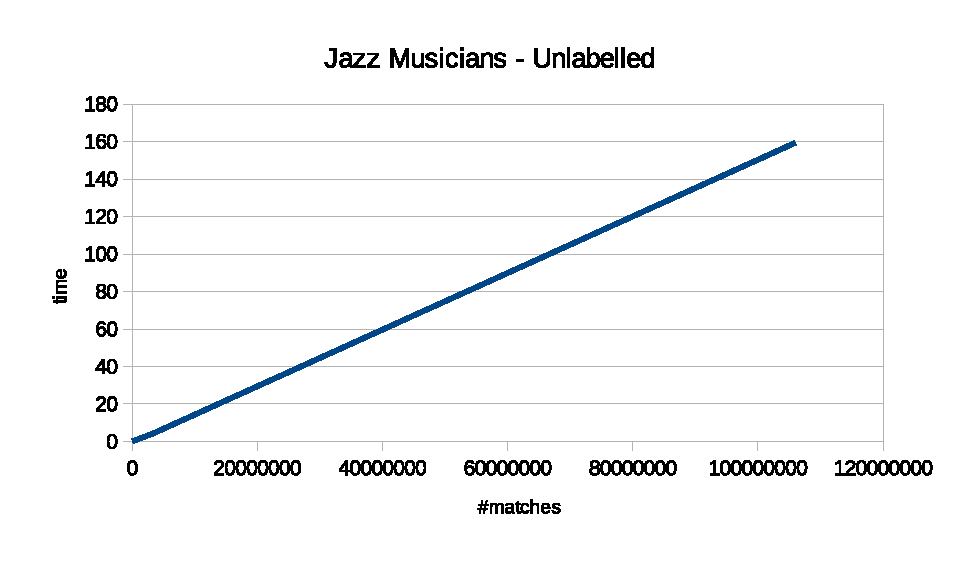
\includegraphics[scale=0.55]{images/Jazz_unlabelled_tpm.eps}
        \caption*{(b) time vs \#matches}       
    \end{minipage}   
\caption{Jazz musicians dataset with unlabelled data and query graphs}
\label{fig:distmx}
\end{figure}

As from the comparison graph in figure 4.1 (a), The parallel implementation runs faster as compared to the sequential version. However, both the implementations take exponential time to get the matches. In figure 4.1 (b), A plot for number of matches vs time elapsed is plotted. The number of matches obtained corresponds to various query graph sizes. We can observe that the time taken per match increases linearly (polynomially).

\begin{figure}[h!]
    \centering
    \begin{minipage}[b]{.45\textwidth}
        \hspace*{-0.5in}
        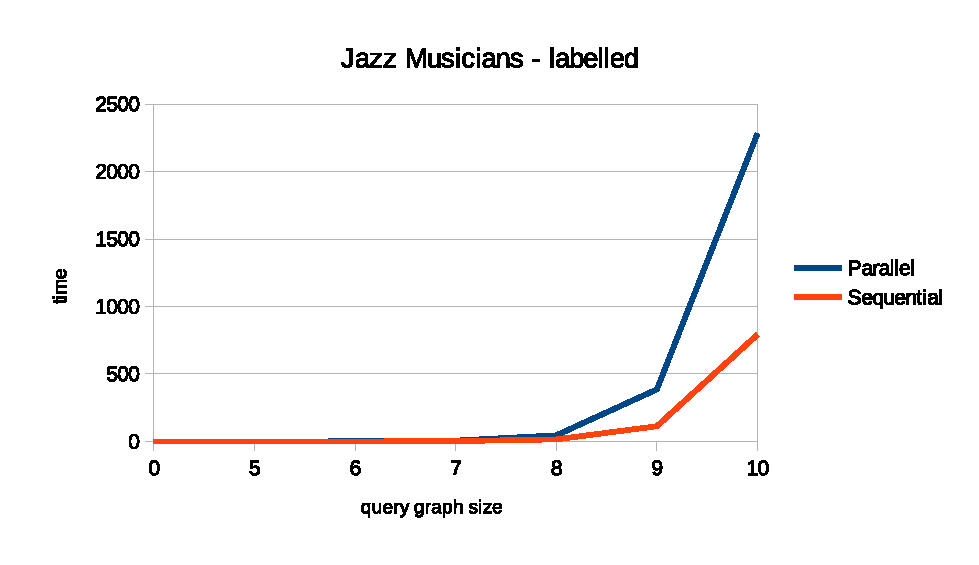
\includegraphics[scale=0.55]{images/Jazz_labelled.eps}
        \caption*{(a) average time vs query graph size}        
    \end{minipage} \hfill  
    \begin{minipage}[b]{.45\textwidth}
        \hspace*{-0.2in}
        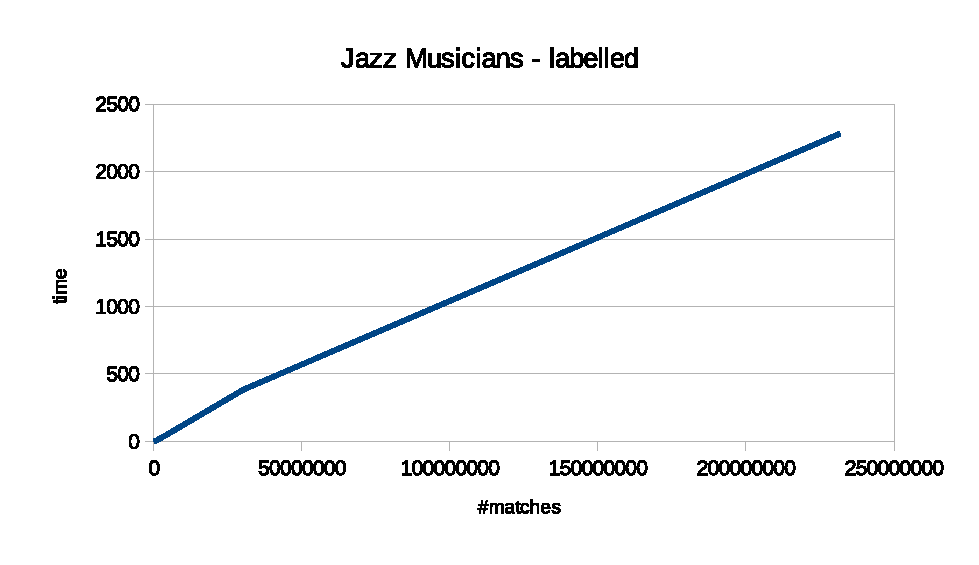
\includegraphics[scale=0.55]{images/Jazz_labelled_tpm.eps}
        \caption*{(b) time vs \#matches}       
    \end{minipage}   
\caption{Jazz musicians dataset with labelled data and query graphs}
\label{fig:distmx}
\end{figure}

For labelled graph, 5 random labels were assigned to the data and the query graphs. In this case, the performance of sequential implementation is better as compared to the parallel implementation. This is because in case of labelled graphs, the number of candidates of each node reduces. Because of which the
number of threads and hence the amount of parallelism decreases.

The algorithms were also compared on labelled data graph and dense labelled query graphs (both with 3 labels). But the result was similar as the sparse query graph.

\begin{figure}[]
\begin{center}
        \centering
        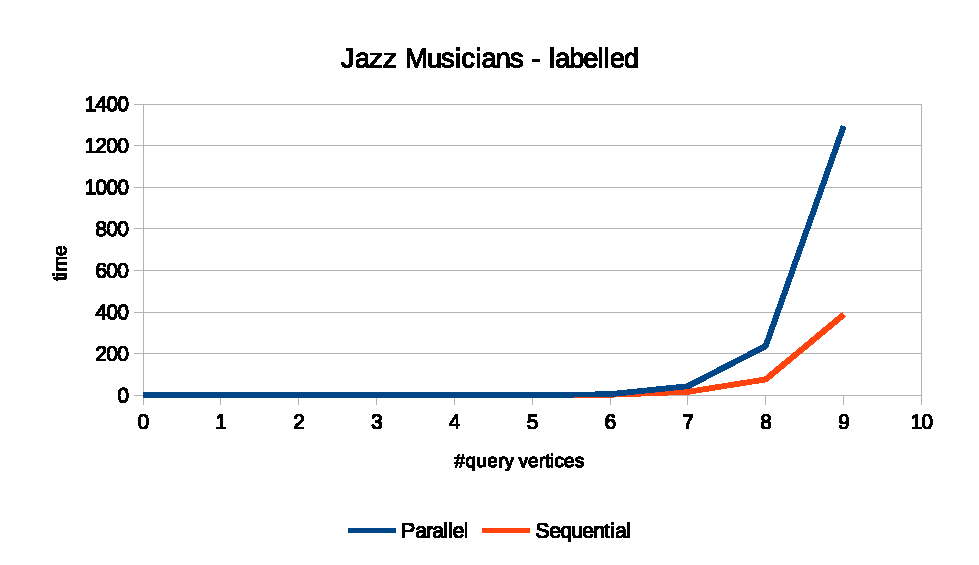
\includegraphics[width=0.7\textwidth]{images/jazz_unlabelled_dense.eps}
        \caption{\textsc{SubgraphSearch}}
        \label{fig:flowchart}
\end{center}
\end{figure}

\section{Dataset: Hamsterster friendships}

Source of this dataset is \cite{hasmtersert}. This graph represents network of friendship between users on the website hamsterster.com. The graph contains 1858 vertices and 12534 edges with a maximum degree of 272 edges and an average degree of 13.492 edges / vertex. Following plot shows the results of parallel and sequential implementation on the unlabelled graph.

\begin{figure}[H]
    \centering
    \begin{minipage}[b]{.45\textwidth}
        \hspace*{-0.5in}
        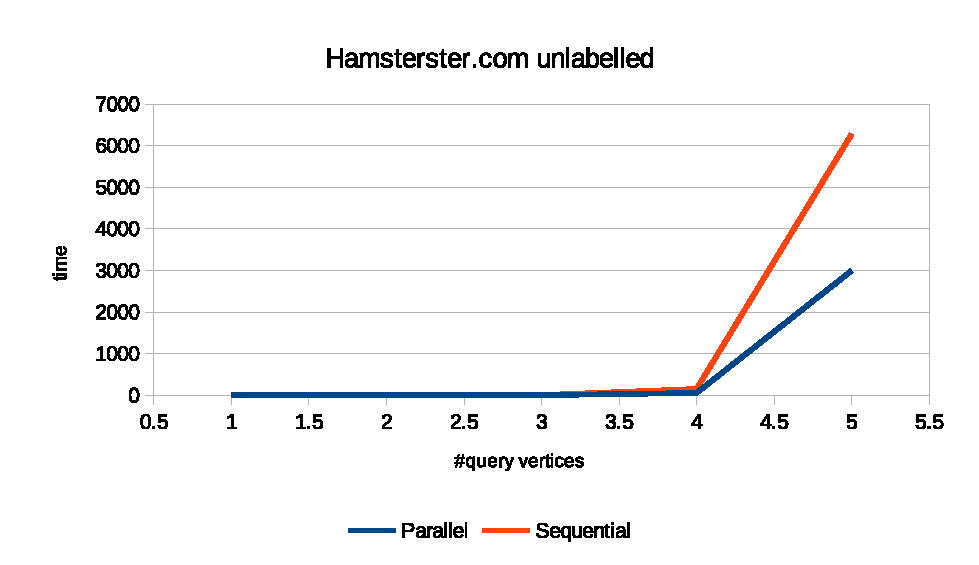
\includegraphics[scale=0.55]{images/hamsterster_unlabelled.eps}
        \caption*{(a) average time vs query graph size}        
    \end{minipage} \hfill  
    \begin{minipage}[b]{.45\textwidth}
        \hspace*{-0.2in}
        \includegraphics[scale=0.55]{images/hamsterster_unlabelled_tpm.eps}
        \caption*{(b) time vs \#matches}       
    \end{minipage}   
\caption{Hamsterster friendship dataset with unlabelled data and query graphs}
\label{fig:distmx}
\end{figure}

Since this graph is larger as compared to the jazz musicians graph, the number of candidates and hence the number of threads launched is more. Evidently, the performance of the parallel implementation is better than the sequential implementation. Also the average time elapsed per match is again linear.

As for the labelled graphs (5 labels), the performance of both the sequential and parallel versions are similar with the parallel implementation outperforming the sequential implementation for query sizes below 5 vertices.


\begin{figure}[H]
    \centering
    \begin{minipage}[b]{.45\textwidth}
        \hspace*{-0.5in}
        \includegraphics[scale=0.55]{images/hamsterster_labelled.eps}
        \caption*{(a) average time vs query graph size}        
    \end{minipage} \hfill  
    \begin{minipage}[b]{.45\textwidth}
        \hspace*{-0.2in}
        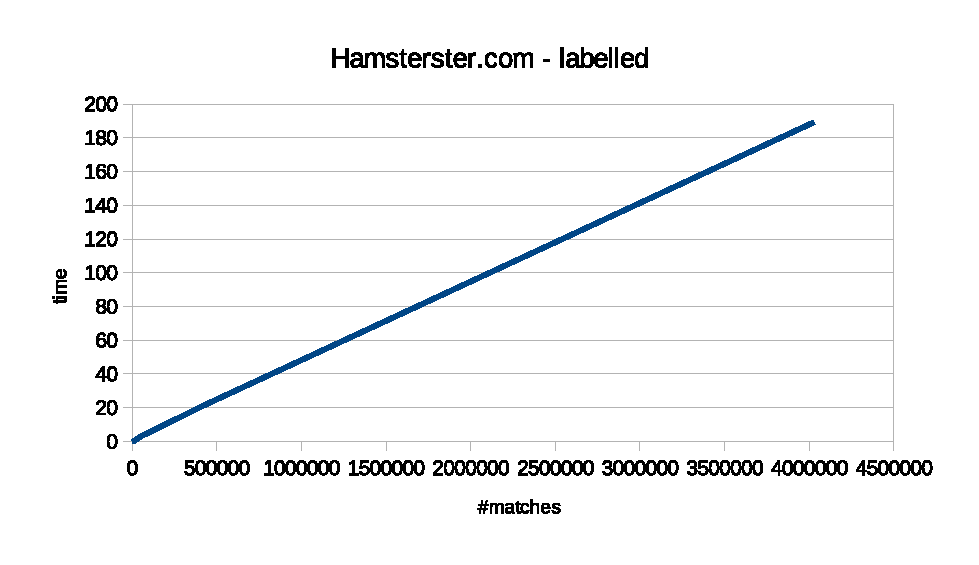
\includegraphics[scale=0.55]{images/hamsterster_labelled_tpm.eps}
        \caption*{(b) time vs \#matches}       
    \end{minipage}   
\caption{Hamsterster friendship dataset with labelled data and query graphs}
\label{fig:distmx}
\end{figure}

\section{Dataset: US power grid}

Source of this dataset is \cite{powergrid}.This dataset contains the contains information on connectivity of the power grid of Western United States. Each node represents either a generator, a transformer or a substation. Each edge of the graph represents a wire connecting either of these. This graphs has 4941 vertices, 6594 edges and the maximum degree of a node is 19 edges. Since this a relatively sparse graph with an average degree of 2.6691 edges / vertex, the query graphs used on this data graph is relatively sparse in order to get sufficient number of matches.

Figure 4.6 (a) shows the comparison between performance of serial and parallel implementation of the algorithms over unlabelled data and query graphs.

\begin{figure}[h!]
    \centering
    \begin{minipage}[b]{.45\textwidth}
        \hspace*{-0.5in}
        \includegraphics[scale=0.55]{images/USpower_unlabelled.eps}
        \caption*{(a) average time vs query graph size}        
    \end{minipage} \hfill  
    \begin{minipage}[b]{.45\textwidth}
        \hspace*{-0.2in}
        \includegraphics[scale=0.55]{images/USpower_unlabelled_tpm.eps}
        \caption*{(b) time vs \#matches}       
    \end{minipage}   
\caption{US power grid dataset with unlabelled data and query graphs}
\label{fig:distmx}
\end{figure}

The performance of parallel implementation is better as compared to the sequential implementation for this dataset. The number of vertices in this graph is larger than the previous two graphs. The number of threads launched in the execution of parallel version for unlabelled graph is 3715.

Figure 4.7 (a) shows the comparison between performance of serial and parallel implementation of the algorithms over labelled data and query graphs. Since each node in the graph can either be a generator, a transformer or a substation, 3 labels are used for the labelled graph which are randomly assigned to the nodes.

\begin{figure}[h!]
    \centering
    \begin{minipage}[b]{.45\textwidth}
        \hspace*{-0.5in}
        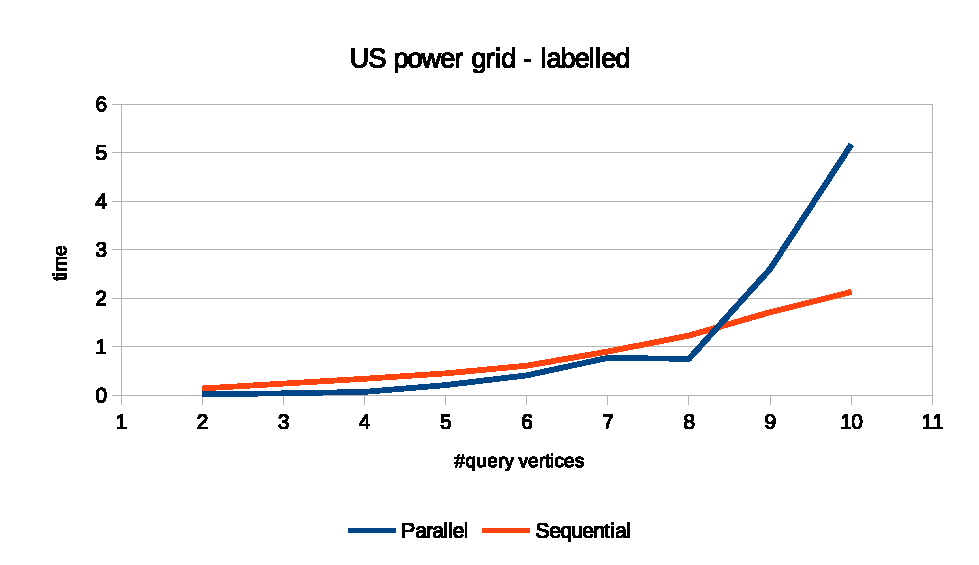
\includegraphics[scale=0.55]{images/USpower_labelled.eps}
        \caption*{(a) average time vs query graph size}        
    \end{minipage} \hfill  
    \begin{minipage}[b]{.45\textwidth}
        \hspace*{-0.2in}
        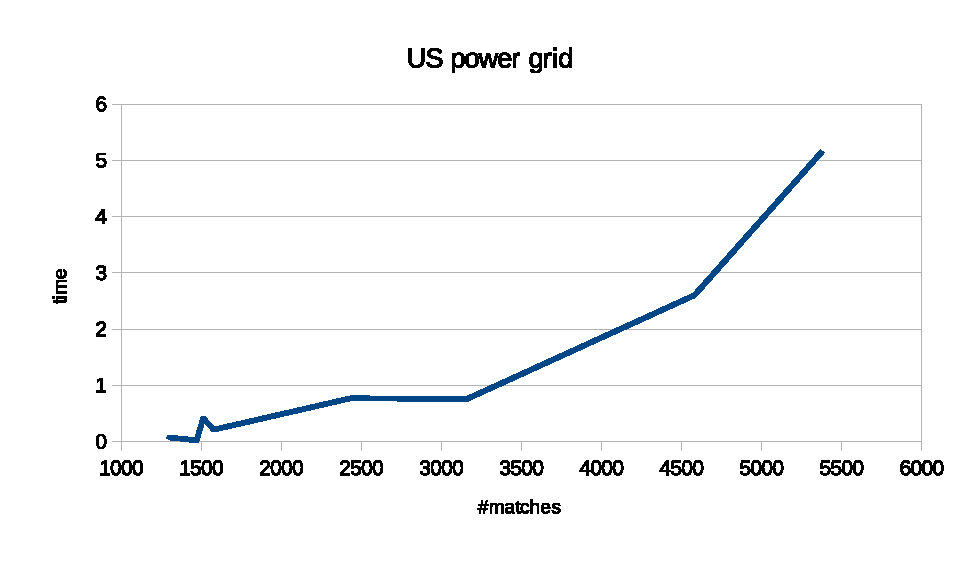
\includegraphics[scale=0.55]{images/USpower_labelled_tpm.eps}
        \caption*{(b) time vs \#matches}       
    \end{minipage}   
\caption{US power grid dataset with labelled data and query graphs}
\label{fig:distmx}
\end{figure}

In the labelled case, the parallel implementation performs better for query graph size $\leq$ 8. This is because, the number of candidates of each node decreases drastically with the increase in size of query vertex (given that data graph is very sparse). Another observation in this case is the irregular time / match curve. This is due to the fact that the number of matches is not monotonically increasing with the increase in query graph size, as was the case with all the previous graphs. The number of matches obtained for query size 2, 3, 4, 5 and 6 were 1472, 1299, 1303, 1580 and 1513 respectively.

\section{Dataset: Chicago Transportation}

Source of this dataset is \cite{chicago}. This graph represents the transportation routes in Chicago city. The vertices in the graph represent a transportation terminal and an edge represents the connection between two terminals. This is a disconnected and a very sparse graph with 1467 vertices, 1298 edges with an average degree of 1.7696 edges / vertex and a max degree of 12 edges.

For this data graph, very sparse query graphs were used because the less number of matches with dense graphs (mostly 0). The comparison of performance is shown in figure 4.8

\begin{figure}[h!]
    \centering
    \begin{minipage}[b]{.45\textwidth}
        \hspace*{-0.5in}
        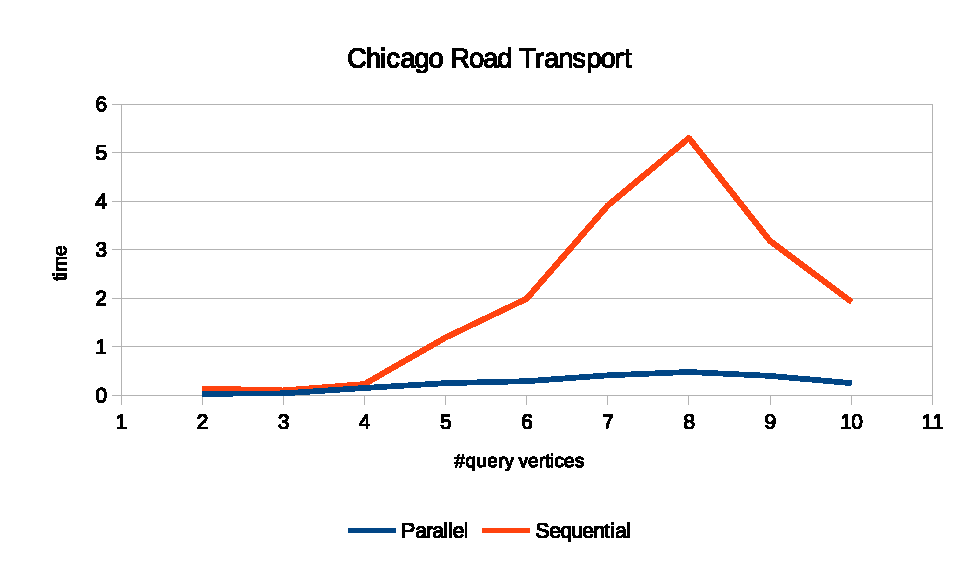
\includegraphics[scale=0.55]{images/chicago_unlabelled.eps}
        \caption*{(a) average time vs query graph size}        
    \end{minipage} \hfill  
    \begin{minipage}[b]{.45\textwidth}
        \hspace*{-0.2in}
        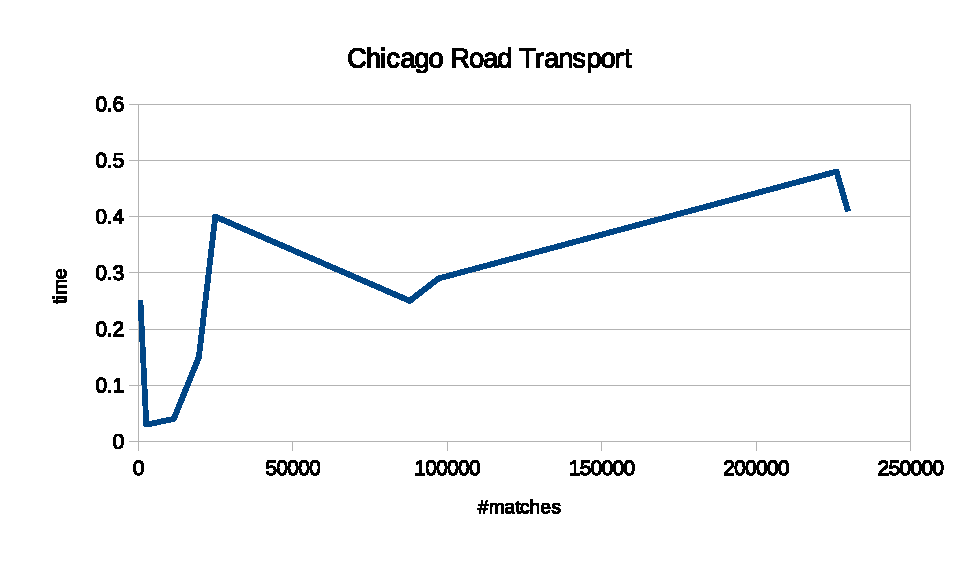
\includegraphics[scale=0.55]{images/chicago_unlabelled_tpm.eps}
        \caption*{(b) time vs \#matches}       
    \end{minipage}   
\caption{Chicago transportation dataset with labelled data and query graphs}
\label{fig:distmx}
\end{figure}

Similar to the US power grid dataset, the time / match curve of this graph is very irregular because of the non monotonocity of the number of matches. For query size 2 to 10 in order, the number of matches are 2596, 11485, 19614, 87886, 97232, 229762, 226072, 24922 and 704. It is evident that the execution time of both the sequential and parallel algorithm depends on the number of matches. However, the parallel implementation outperforms the sequential implementation because of the comparatively large graph size.